\section{Mie Theory}
The scattering problem considered in this work is that arising when an arbitrary beam of light interacts with a spherical particle. As mention in Sec. \ref{sec:2}, we additionally restrict the processes to linear, homogeneous and isotropic particles. This scattering process is often referred to as Mie scattering and is illustrated in Fig. \ref{fig:glmt}. 
\begin{figure}
    \centering
    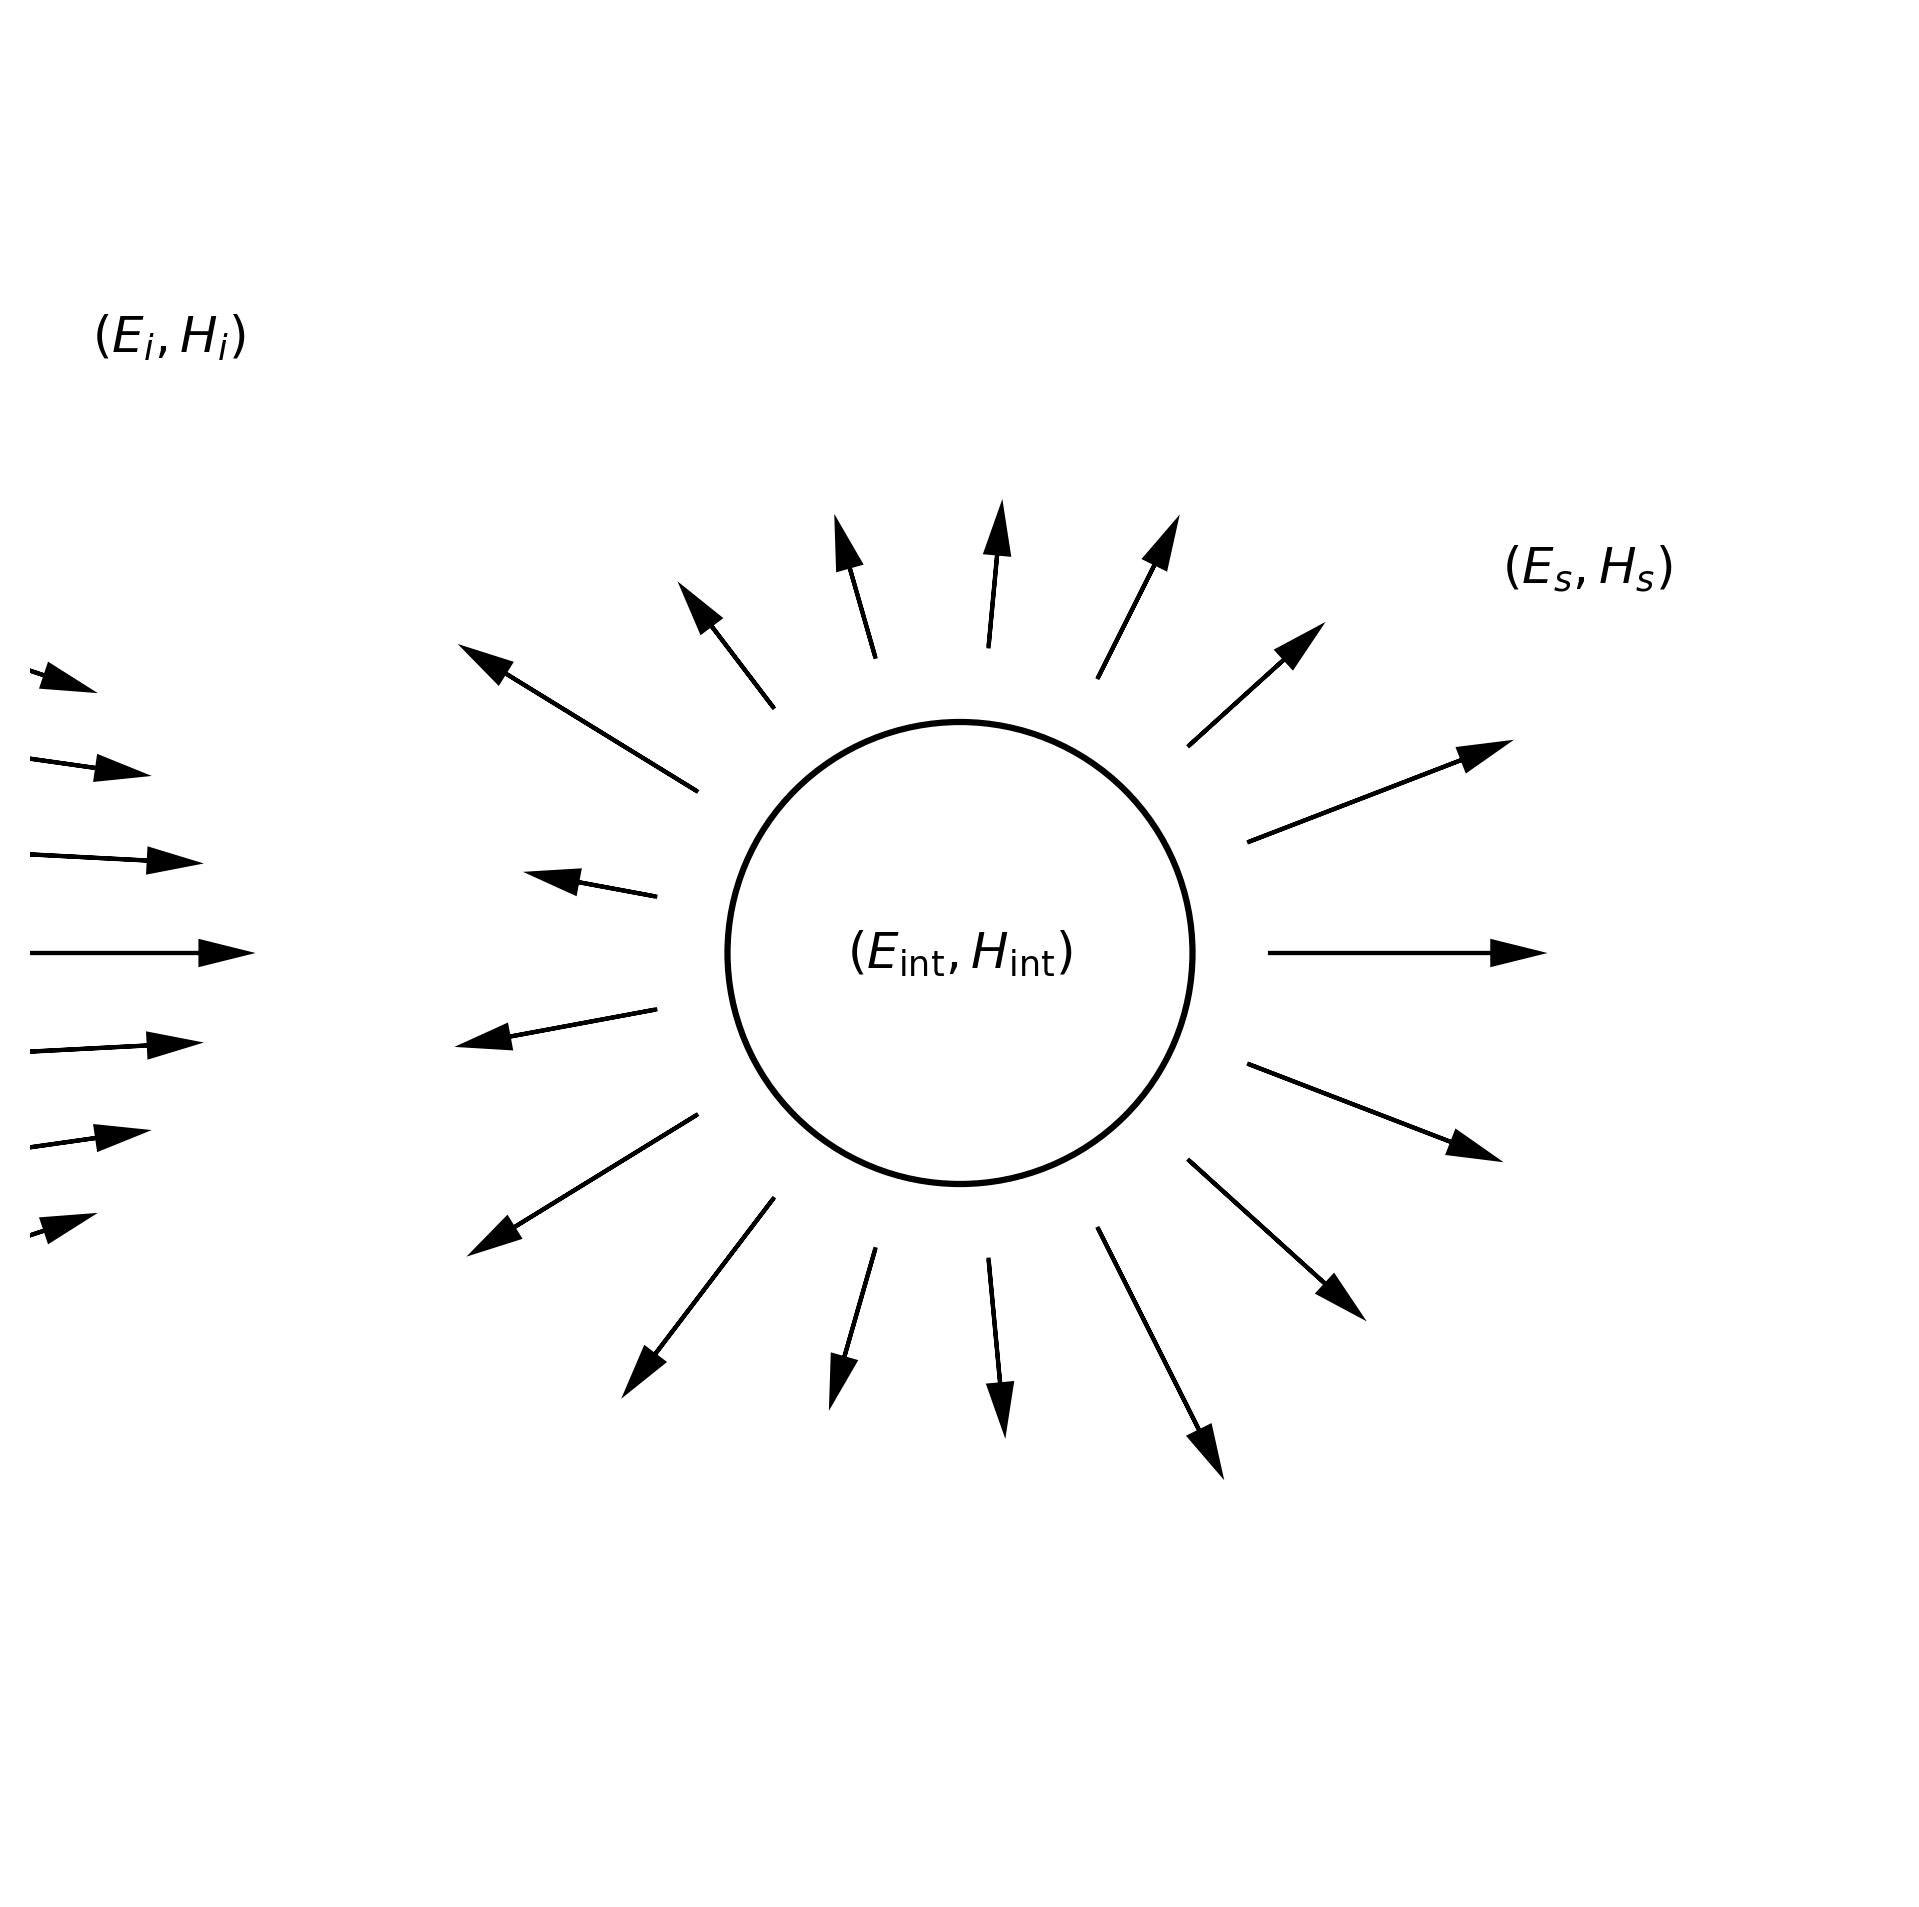
\includegraphics[trim={0 1cm 0 1cm},clip,width=0.6\textwidth]{Figures/figure.png}
    \caption{Illustration of generalized Mie scattering with an arbitrary (here cylindrically symmetric) incident beam. An internal and scattered field is produced in the process.}
    \label{fig:glmt}
\end{figure}
By assuming an incident field of the form in Eq. \ref{eq:E_i_expansion} and applying the electromagnetic boundary conditions, one obtains similar expression for the scattered and internal fields, outside and inside the particle respectively.

\begin{align}
& \mathbf{E}^{\mathbf{s}}=\sum_{j=0}^{\infty}\sum_{m_z=-j}^j b_j g_{jm_z}^{(m)}\mathbf{A}_{j m_z^*}^{(m)}+ a_j g_{jm_z}^{(e)}\mathbf{A}_{j m_z^*}^{(e)}\label{eq:Mie_S} \\
& \mathbf{E}^{\mathrm{int}}=\sum_{j=0}^{\infty}\sum_{m_z=-j}^j c_jg_{jm_z}^{(m)} \mathbf{A}_{j m_z^*}^{(m)}+ d_jg_{jm_z}^{(e)} \mathbf{A}_{j m_z^*}^{(e)}\label{eq:Mie_I},
\end{align}
i.e. simply the same sum but with another coefficient on each term. These are called the Mie coefficients and have the following expressions:
\begin{gather}
a_j=\frac{\mu n_r^2 j_j\left(n_r x\right)\left[x j_j(x)\right]^{\prime}-\mu_1 j_j(x)\left[n_r x j_j\left(n_r x\right)\right]^{\prime}}{\mu n_r^2 j_j\left(n_r x\right)\left[x h_j^{(1)}(x)\right]^{\prime}-\mu_1 h_j^{(1)}(x)\left[n_r x j_j\left(n_r x\right)\right]^{\prime}} \\
b_j=\frac{\mu_1 j_j\left(n_r x\right)\left[x j_j(x)\right]^{\prime}-\mu j_j(x)\left[n_r x j_j\left(n_r x\right)\right]^{\prime}}{\mu_1 j_j\left(n_r x\right)\left[x h_j^{(1)}(x)\right]^{\prime}-\mu h_j^{(1)}(x)\left[n_r x j_j\left(n_r x\right)\right]^{\prime}} \\
c_j=\frac{\mu_1 j_j(x)\left[x h_j^{(1)}(x)\right]^{\prime}-\mu_1 h_j^{(1)}(x)\left[x j_j(x)\right]^{\prime}}{\mu_1 j_j\left(n_r x\right)\left[x h_j^{(1)}(x)\right]^{\prime}-\mu h_j^{(1)}(x)\left[n_r x j_j\left(n_r x\right)\right]^{\prime}} \\
d_j=\frac{\mu_1 n_r j_j(x)\left[x h_j^{(1)}(x)\right]^{\prime}-\mu_1 n_r h_j^{(1)}(x)\left[x j_j(x)\right]^{\prime}}{\mu n_r^2 j_j\left(n_r x\right)\left[x h_j^{(1)}(x)\right]^{\prime}-\mu_1 h_j^{(1)}(x)\left[n_r x j_j\left(n_r x\right)\right]^{\prime}}
\end{gather}  
Here, $x$ is the size parameter, $x=2\pi R/\lambda$, $n_r=n_1/n_0$ is the relative refractive index of the particle ($n_1$) and the medium ($n_0$).\\
In Figs. \ref{fig:scatfig1} \& \ref{fig:scatfig2}, scattering scenarios are plotted for two instances of a $l=3$ incident beam focused with an aplanatic lens with $\mathrm{NA}=0.9$. Note that the incident field is not included, although it would of course be present in an experiment.
The first is an example of a high helicity preservation case mentioned in the next chapter. The second is a resonance in the cross section of the internal EM field. The extent of the scatterer is shown with a white line. The scatterer is illuminated with a focused field like Eq. \ref{eq:Efoc} propagating in $z$. The XY slice is therefore the scatterer along the direction of the beam. In the XZ slice, we see a cylindrically symmetric scattered field from the edge of the particle and the internal field.\\
The internal field in Fig. \ref{fig:scatfig1} has the shape of the toroidally shaped focused beam in the XY plane, while a shell of evenly distributed high intensity is scattered. In the XZ plane we see that this shell is in fact scattered mostly orthorgonally to the propagation of the beam.\\
In the resonant field, Fig. \ref{fig:scatfig2}, one quickly sees that the colour scale has values of three orders of magnitude higher than \ref{fig:scatfig1}. The highest intensities are at $z=\pm 2$. Here, four distinct spots are located at the edge of the scatterer.
% First figure
\begin{figure}[ht]
    \centering
    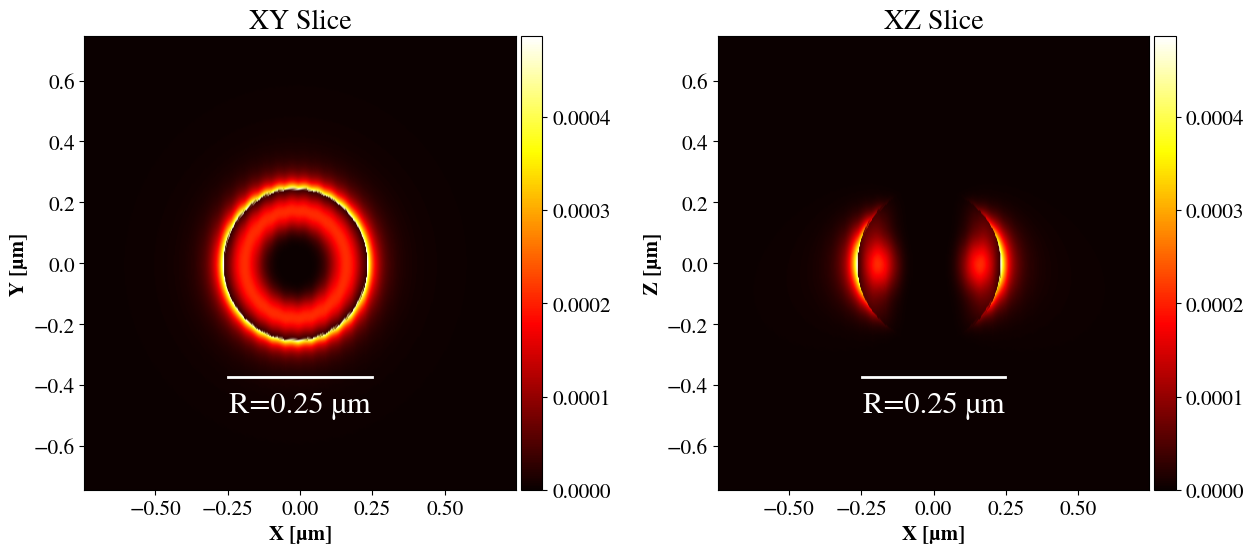
\includegraphics[width=\textwidth]{Figures/scat_pres_l3.png} % Replace with your image
    \caption{Scattered and internal field for a $l=3$ incident beam illuminating a scatterer with refractive index $3.0$ with large helicity preservation}
    \label{fig:scatfig1}
\end{figure}

% Second figure
\begin{figure}[ht]
    \centering
    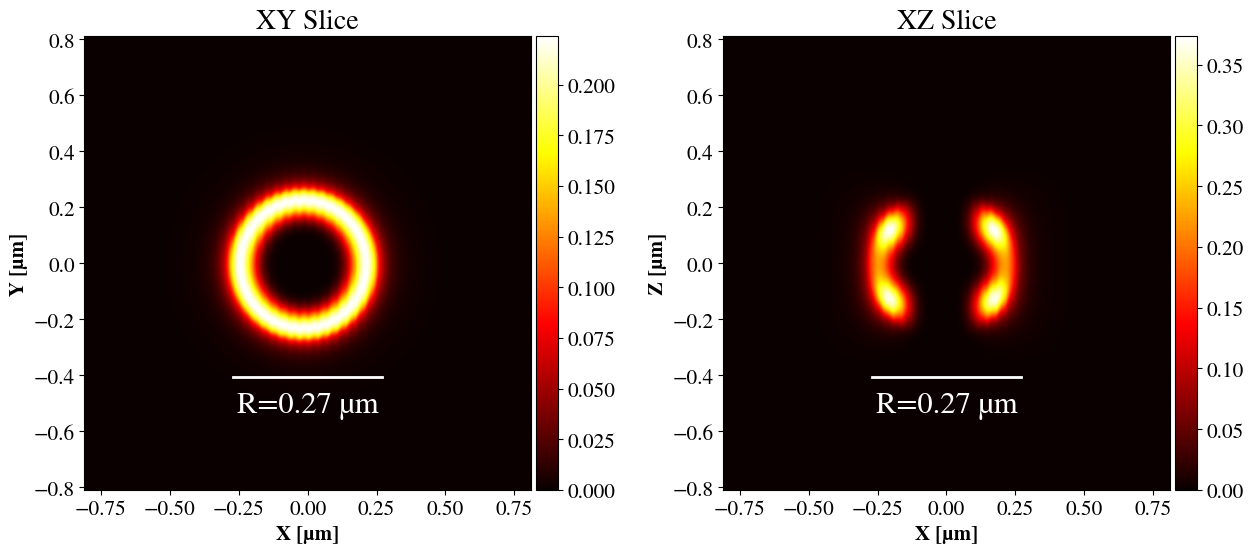
\includegraphics[width=\textwidth]{Figures/scat_res_l3.png} % Replace with your image
    \caption{Scattered and internal field for a $l=3$ incident beam illuminating a scatterer with refractive index $3.0$ at resonance.}
    \label{fig:scatfig2}
\end{figure}
